\documentclass[aps,prd,preprint]{revtex4-1}
\usepackage{graphicx}
\usepackage{amsfonts,amsmath,amssymb}
\usepackage{dsfont}
\usepackage{nccmath}
\usepackage{fnbreak}
\usepackage{float}
\usepackage{listings}

\begin{document}

\newcommand{\christoffel}[3]{
    \left\{ \begin{matrix} #1 \\ #2 #3 \end{matrix} \right\}
}

\title{On The Dynamics Of The Gravitational Field And Higher Order Field Equations}
\author{D.E. Thomas}
\date{\today}

\begin{abstract}
    Einstein's General Relativity, while extraordinarily successful in explaining gravitational phenomena, faces challenges addressing certain cosmological observations demonstrated by galaxy roation curves and the expansion of the universe. 2014 Poplawski presented a higher order model of gravitation that reframes the gravitational field in terms of the connection, with the curvature tensor as the field strength. I reconsider the action in this model is based on the squared norm of the field strength. Through analysis of the Euler-Lagrange equations, particularly focusing on the metric equations, I demonstrate that Einstein's field equations emerge as a limiting case within a more comprehensive framework. Analyzing the field equations of the gravitational field, as the connection, I calculate corrections. Global corrections produce a term that replaces the dark energy sector with a geometric term. Local corrections take the form of a Yukawa potential. D'Agostino et al. showed that a Yukawa correction can account for the rotational velocities of galaxies without dark matter. Thus this broader framework provides explanations for observed experimental discrepancies without exotic materia, while maintaining consistency with established gravitational phenomena.
\end{abstract}

\maketitle

\section*{Introduction}

Einstein's field equations (EFEs), the cornerstone of General Relativity (GR), have stood as one of the most profound and successful descriptions of gravity for over a century. These elegant equations relate the geometry of spacetime to the distribution of matter and energy within it, providing a framework for understanding gravitational phenomena with a precision far exceeding that of any model previous to their conception~\cite{Einstein_1916,misner_2017}.

However, as our observational capabilities have advanced and our theoretical understanding has deepened, several critical challenges to the completeness of the EFEs have emerged. These challenges span both the cosmic and quantum scales, highlighting the need for a more comprehensive theory of gravity~\cite{brandes_2013}.

The Cosmological Constant Problem: A staggering discrepancy of significant orders of magnitude exists between quantum field theory predictions for vacuum energy and the observed cosmological constant. This discrepancy has been dubbed ``the worst theoretical prediction in the history of physics''. It suggests a fundamental gap in our understanding of how vacuum energy interacts with gravity at cosmological scales~\cite{weinberg_1989,hobson_2006}.

Dark Matter and Dark Energy: The necessity of dark matter to explain galactic rotation curves and dark energy to account for the universe's accelerating expansion suggests that the EFEs may not fully describe gravitational phenomena on cosmological scales. These additional components, constituting most of the universe's content, are not predicted by the original equations~\cite{bertone_2018,frieman_2008}. This discrepancy points to a significant incompleteness in our current gravitational theory.

Quantum Gravity: The EFEs, while extraordinarily successful in describing gravity at macroscopic scales, are fundamentally classical in nature. They do not incorporate quantum mechanics, leading to breakdowns at very small scales and high energies, such as those found in black holes or the early universe. Moreover, GR has resisted attempts at quantization, suggesting that a more fundamental theory—one that is naturally amenable to quantization and renormalization—may be necessary~\cite{wald_1984,rovelli_2004,hawking_1973}.

In 2014 Poplawski presented a reframing of Einstein's original GR by taking the connection by itself, without assuming a prior metric, is the fundamental dynamical variable for gravitation and the field strength is built from the curvature and torsion of that connection. The Lagrangian is constructed purely in terms of the connection (via its curvature and torsion), not assuming a metric in advance. This formulation reframes gravity more in terms of connection and curvature, rather than metric first~\cite{poplawski_2014}.

In this paper, I consider Poplawski's mathematical framework that builds upon Einstein's foundational work while addressing these critical challenges. My approach aims to reconcile the observed cosmological differences with theoretical predictions without resorting to the introduction of exotic forms of matter or energy.

In the following section I will reintroduce the mathematical framework, which extends the EFEs in a way that naturally accommodates the observed cosmological phenomena and paves the way for a more complete description of gravitational interactions across all scales.

\section{From Einstein to a modern field theory}
\subsection*{A Resume of General Relativity}
When Einstein first wrote down the field equations of his general theory of relativity in action form, he proposed the Lagrangian~\cite{Einstein_1915,Einstein_1916},
\begin{equation}\label{Einstein_1915}
    L = g^{\mu\nu} \christoffel{\alpha}{\mu}{\beta} \christoffel{\beta}{\nu}{\alpha}
\end{equation}
where $g^{\mu\nu}$ is the metric tensor and $\christoffel{\alpha}{\mu}{\beta}$ is the Christoffel symbol defined as,
\begin{equation}\label{christoffel}
    \christoffel{\alpha}{\mu}{\beta} = \frac{1}{2} g^{\alpha\sigma} \left(\partial_{\beta}g_{\sigma\mu} + \partial_{\mu}g_{\sigma\beta} - \partial_{\sigma}g_{\mu\beta}\right)
\end{equation}

Later, Einstein, Hilbert, and others reformulated the action of the theory as~\cite{Hilbert_1915,misner_2017},
\begin{equation}\label{Einstein-Hilbert_action}
    S=\int{R \sqrt{-g} d^4x}
\end{equation}
where $R = R^{\alpha}_{\mu\beta\nu}g^{\beta}_{\alpha}g^{\mu\nu}$, \\
$R^{\alpha}_{\mu\beta\nu}$ is the Riemann curvature tensor, \\
$R$ is the curvature scalar, \\
$g$ is the determinant of the metric, $\sqrt{-g} d^4x$ the canonical invariant volume element on a manifold.
Varying this action with respect to the metric tensor yields the field equations,
\begin{equation}\label{EFEs}
    R^{\alpha}_{\mu\beta\nu}g^{\beta}_{\alpha} = R_{\mu\nu} = 0
\end{equation}
here, $R_{\mu\nu}$ is called the Ricci curvature tensor.

This result, however, was derived assuming that the spacetime is torsion-free~\cite{Einstein_1915,Einstein_1916,misner_2017,watanabe_2004}. Including torsion $\mathcal{T}$ (defined by double of the antisymmetric part of the connection in its last two indices, i.e. $\mathcal{T}^{\alpha}_{\mu\nu}=\Gamma^{\alpha}_{\mu\nu} - \Gamma^{\alpha}_{\nu\mu}$), the full affine connection is expressed as,
\begin{equation}\label{affine_connection}
    \Gamma^{\alpha}_{\mu\nu}=\frac{1}{2}g^{\alpha\sigma}(\partial_{\nu}g_{\sigma\mu}+\partial_{\mu}g_{\sigma\nu}-\partial_{\sigma}g_{\mu\nu} + \mathcal{T}_{\sigma\mu\nu}+\mathcal{T}_{\mu\nu\sigma}-\mathcal{T}_{\nu\sigma\mu})
\end{equation}
In any holonomic basis, the affine connection completely describes the covariant derivative up to metric compatibility~\cite{misner_2017}. Recognizing this, Cartan showed that varying the action of GR with respect to torsion yields the torsion tensor field equations~\cite{cartan_1922},
\begin{equation}\label{cartan_field_eq}
    \mathcal{T}^{\alpha}_{\mu\nu} + g^{\alpha}_{\mu}\mathcal{T}^{\sigma}_{\nu\sigma} - g^{\alpha}_{\nu}\mathcal{T}^{\sigma}_{\mu\sigma} = 0
\end{equation}

Here one must find themselves at a crossroads. The field equations of Einstein-Cartan theory (\ref{EFEs} \& \ref{cartan_field_eq}) are found by varying with respect to the two parts of the connection independently, while treating the metric and torsion each as gravitational potential fields. One should ask: why not treat the entire affine connection as the gravitational potential and find an invariant action to vary with respect to the field represented by the affine connection?

Poplawski~\cite{poplawski_2014} used the same Einstein-Hilbert action but varied with respect to the affine connection. However, an action can be constructed in a form similar to that seen in other field theories. Specifically, I take a first-order derivative of the dynamic field and square it appropriately so as to ensure invariance with respect to some local symmetry~\cite{peskin_1995,weinberg_1995}, in this case, general coordinate transformations.

In examining equation~\eqref{Einstein_1915}, I notice it appears that Einstein may have initially approached his model with this squared first derivative formulation in some manner, considering he treated the metric as the gravitational potential. However, given the limited exploration and popularization of this approach at the time, it is understandable that he was persuaded to adopt a more minimal scalar quantity. While this historical interpretation is intriguing, it is purely speculative on my part and not well-documented.

\subsection*{Construction of The Affine Field Equations}
I will start with the affine connection and take a derivative as follows,
\begin{equation}
    \mathcal{R}^\alpha_{\mu\beta\nu} = \partial_{\beta}\Gamma^{\alpha}_{\nu\mu}-\partial_{\nu}\Gamma^{\alpha}_{\beta\mu}+\Gamma^{\alpha}_{\beta\sigma}\Gamma^{\sigma}_{\nu\mu} - \Gamma^{\alpha}_{\nu\sigma}\Gamma^{\sigma}_{\beta\mu} + \Gamma^{\sigma}_{\beta\nu}\Gamma^{\alpha}_{\sigma\mu}-\Gamma^{\sigma}_{\nu\beta}\Gamma^{\alpha}_{\sigma\mu}
\end{equation}
$\mathcal{R}^\alpha_{\mu\beta\nu}$ is the complete curvature tensor in the presence of torsion or any other antisymmetric contributions to the connection~\cite{watanabe_2004}.
\begin{equation}
    \mathcal{R}^\alpha_{\mu\beta\nu}=R^{\alpha}_{\mu\beta\nu}+\mathcal{T}^{\sigma}_{\beta\nu}\Gamma^{\alpha}_{\sigma\mu}
\end{equation}
Let us define $\mathcal{R}^\alpha_{\mu\beta\nu}$ as the gravitational field strength. The Lagrangian density will be built from the field strength in a manner similar to modern geometric field theories~\cite{peskin_1995,weinberg_1995}, by taking the inner product of the field strength with itself,
\begin{equation}\label{higher_order_action}
    S=\int{\mathcal{R}^\alpha_{\mu\beta\nu}\mathcal{R}_\alpha^{\mu\beta\nu}D^4x}
\end{equation}
where $D^4x$ is a generalized invariant volume form.
This Lagrangian and its associated Euler-Lagrange equations with respect to the gravitational field $\Gamma$ will yield the gravitational field equations,
\begin{equation}\label{euler-lagrange}
    \frac{\partial}{\partial\Gamma^{\alpha}_{\nu\mu}}\left(\mathcal{R}^\alpha_{\mu\beta\nu}\mathcal{R}_\alpha^{\mu\beta\nu}\right) - \partial_{\rho}\frac{\partial}{\partial(\partial_{\rho}\Gamma^{\alpha}_{\nu\mu})}\left(\mathcal{R}^\alpha_{\mu\beta\nu}\mathcal{R}_\alpha^{\mu\beta\nu}\right) = 0
\end{equation}
the {\it field equations\/} are,
\begin{equation}\label{higher_order_field_eq}
    D_\beta \mathcal{R}_\alpha^{\mu\beta\nu} = 0
\end{equation}
where $D_\alpha$ is the covariant derivative with respect to the curved connection with torsion.

In addition to the field equations, one must pair with {\it equations of motion\/} to provide a description of the motion of a test particle in the field solved for in the field equations. In Einstein's general theory of relativity, the geodesic equation serves the role of this equation of motion~\cite{hauser_2019_1,hauser_2019_2,hauser_2019_3},
\begin{equation}\label{geodesic_equation}
    \frac{d^2x^\mu}{d\lambda^2} + \Gamma^{\mu}_{\alpha\beta}\frac{dx^\alpha}{d\lambda}\frac{dx^\beta}{d\lambda} = 0
\end{equation}
This is found by varying the path interval with respect to the position of a free particle. In the model presented here, the path interval for a free particle is given by,
\begin{equation}\label{free_particle_action}
    S = \int mc^2 D\lambda
\end{equation}
where $D\lambda$ is an invariant path element such that,
\begin{equation}
    D\lambda \rightarrow \frac{D\lambda}{dx^\mu}dx^{\mu} \rightarrow d\lambda + \Gamma^{\mu}_{\mu\nu}\frac{dx^{\nu}}{d\lambda}d\lambda
\end{equation}
This is equivalent to the canonical invariant element ($\sqrt{-g}d\lambda$) in this case, but more generalized if extended and easier to work with below. Varying with respect to $x^{\mu}$, one finds,
\begin{equation}\label{geodesic_deviation}
    \frac{d^2 x^\alpha}{d\lambda^2} + R^{\alpha}_{\beta\mu\nu}\frac{dx^\beta}{d\lambda}\frac{dx^\mu}{d\lambda}X^{\nu} = 0
\end{equation}
where $X$ is the seperation vector between events on geodesics, this is canonically called the geodesic deviation~\cite{philipp_2015,ganiou_2016}.

\section{Metric Field Equations of the Squared Norm}
\subsection*{Field Equations of the Metric}
The model presented establishes the gravitational field equations and equations of motion. However, in Einstein's GR he considers the metric field equations~\cite{Einstein_1915,Einstein_1916}. I will examine the metric field equations in the presented model to compare with Einstein's equations and present any corrections to the Einstein model in the regime where it could be considered a valid approximation.

Using the action based on the field Lagrangian density $\mathcal{R}^\alpha_{\mu\beta\nu}\mathcal{R}_\alpha^{\mu\beta\nu}$, we can also derive the field equations of the metric,
\begin{equation}\label{higher_order_metric_equations}
    2 D_{[a} D_{b]} \mathcal{R}^{nmab} + \mathcal{R}_{ab} \mathcal{R}^{namb} = 0
\end{equation}
for a detailed derivation of these metric field equations using a variational principle approach see Appendix~\ref{app.derv_metric_field_eqs}.

In the rest of this paper I will generalize the notion of the curvautre tensor such that I refer to $\mathcal{R}$ as the Riemann tensor, it's contraction the Ricci tensor, and the trace of this form of the Ricci tensor as the curvature scalar.

\subsection*{The Einsteinian Limit}
Under what conditions would one expect this to reduce to the Einstein equations, where we can consider the Einstein equations as an approximation? I expect that the Einstein equations would emerge as a weak field limit of~\eqref{higher_order_metric_equations}, when the local curvature becomes negligible. I would not necessarily restrict the global curvature, however. These conditions correspond to a maximally symmetric space, i.e., where the curvature is isotropic and homogeneous everywhere in the universe~\cite{duggal_2013,emparan_2002,jizba_2020}. This would imply that in regions where the gravitational field is weak, we can ignore local effects on the geometry and focus on the solutions for the global geometry~\cite{stephani_2009}, which I hypothesize can be reduced to Einstein's equations.

In a maximally symmetric space the metric is not a function of space, and in a nearly maximally symmetric space the metric can be decomposed into a maximally symmetric background and a local part,
\begin{equation}\label{metric_decomp}
    g_{ab}(x) = \eta_{ab} + h_{ab}(x)
\end{equation}
where $\eta$ is the maximally symmetric metric (this could be $\eta^0$ the metric of a `flat' Minkowski spacetime, $\eta^+$ the metric of a `positively curved' de Sitter space, or $\eta^-$ the metric of a `negatively curved' anti-de Sitter space). The global geometry of spacetime is captured in $\eta$ and the local geometry is described by $h(x)$. This approach, the background field method, is commonly used in perturbative treatments of gravity and quantum field theory in curved spacetime~\cite{hollands_2002,bern_2002}. It allows us to separate the large-scale structure of spacetime from local fluctuations or perturbations. The term $h(x)$ represents small deviations from the maximally symmetric background. In the context of GR, these deviations represent localized gravitational effects. Most commonly, these localized effects are used to describe gravitational waves~\cite{Einstein_1937}. I do not take that wave interpretation here since gravitational waves should be fully described by the gravitational field equations for $\Gamma$. Instead, I view this as local deviations from the background metric due to the local mass content in a region of spacetime.

The Riemann tensor can be decomposed in general~\cite{wheeler_2018},
\begin{equation}\label{Weyl_decomp}
    \mathcal{R}_{abcd} = C_{abcd} + \frac{1}{2} \left( g_{a[c} \mathcal{R}_{d]b} - g_{b[c} \mathcal{R}_{d]a} \right) - \frac{1}{6} g_{a[c} g_{d]b} \mathcal{R}
\end{equation}
where $C_{abcd}$ is canonically called the Weyl tensor. The Weyl tensor vanishes in maximally symmetric spaces~\cite{hofmann_2013}, so one obtains,
\begin{equation}
    \mathcal{R}_{abcd}(\eta) = \frac{1}{2} \left( \eta_{a[c} \mathcal{R}_{d]b}(\eta) - \eta_{b[c} \mathcal{R}_{d]a}(\eta) \right) - \frac{1}{6} \eta_{a[c} \eta_{d]b} \mathcal{R}
\end{equation}
furthermore, the Ricci tensor in a maximally symmetric space is trivially $\mathcal{R}_{ab}(\eta) = \frac{1}{4}\eta_{ab}\mathcal{R}$. Therefore, the Riemann tensor in a maximally symmetric space becomes,
\begin{equation}\label{maximally_symmetric_Riemann}
    \mathcal{R}_{abcd}(\eta) = \frac{1}{12} \eta_{a[c} \eta_{d]b} \mathcal{R}
\end{equation}
thus, the field equations can be simplified as follows,
\begin{equation}
    2 D_{[a} D_{b]} \left( \frac{1}{12} \eta^{n[m} \eta^{a]b} \mathcal{R} \right) + \left( \frac{1}{4}\eta_{ab}\mathcal{R} \right) \left( \frac{1}{12} \eta^{n[a} \eta^{m]b} \mathcal{R} \right) = 0
\end{equation}
notice that neither $\eta$ nor $\mathcal{R}$ are functions of space in this context, and therefore the derivative term vanishes,
\begin{equation*}
    D_{[a} D_{b]} \left( \eta^{n[m} \eta^{a]b} \mathcal{R} \right) = 0
\end{equation*}
the remaining part of the field equations must then also vanish in this context,
\begin{equation*}
    \left( \frac{1}{4}\eta_{ab}\mathcal{R} \right) \left( \frac{1}{12} \eta^{n[a} \eta^{m]b} \mathcal{R} \right) = 0
\end{equation*}
\begin{equation}
    \frac{1}{16} \eta^{nm} \mathcal{R}^2 = 0
\end{equation}

The proposal of Einstein's equations as a weak-field limit under these conditions would imply the following,
\begin{equation}\label{corrections_to_Einstein}
    \frac{1}{16} \eta^{ab} \mathcal{R}^2 = G^{ab} + H^{ab}
\end{equation}
where $G^{ab}$ is the Einstein tensor, and $H^{ab}$ represents a correction. The Einstein tensor in a maximally symmetric vacuum~\cite{wheeler_1986} is given by,
\begin{equation}\label{maximally_symmetric_vacuum_Einstein}
\begin{aligned}
    G^{ab}(\eta) &= \mathcal{R}^{ab}(\eta) \\
    &= \frac{1}{4}\eta^{ab}\mathcal{R}
\end{aligned}
\end{equation}
from equations~\ref{corrections_to_Einstein} and~\ref{maximally_symmetric_vacuum_Einstein} one can conclude that,
\begin{equation*}
    H^{ab} = \frac{1}{16} \eta^{ab} \mathcal{R}^2 - \frac{1}{4}\eta^{ab}\mathcal{R}
\end{equation*}
\begin{equation*}
    H^{ab} = \frac{1}{4} \eta^{ab} \mathcal{R} \left( \frac{\mathcal{R}}{4} - 1 \right)
\end{equation*}
\begin{equation}\label{solved_for_correction}
    H^{ab} = \mathcal{R}^{ab} \left( \frac{\mathcal{R}}{4} - 1 \right)
\end{equation}
when Einstein's equations do not require correections $H^{ab} \approx 0$ and the right hand side of~(\ref{solved_for_correction}) should also vanish,
\begin{equation}
    \mathcal{R}^{ab} \left( \frac{\mathcal{R}}{4} - 1 \right) \approx 0
\end{equation}
therefore either,
\begin{equation*}
    \mathcal{R}\eta^{ab} \approx 0
\end{equation*}
\begin{center}
    or
\end{center}
\begin{equation*}
    \frac{\mathcal{R}}{4} - 1 \approx 0
\end{equation*}
however, since the metric is not generally null either the scalar curvature is vanishing, $\mathcal{R} \approx 0$, or $\mathcal{R} \approx 4$, for Einstein's field equations to require no corrections.

\section{Comparison to Empirical Cosmology}
\subsection*{Global Curvature and Dark Energy}
On scales large enough that the maximally symmetric condition holds, one can examine the differences in the expected and observed average curvature of the universe in the form of the cosmological constant $\Lambda$. Since this is an observed quantity, slightly positive number near zero~\cite{bertone_2018}, I expect the correction $H$ might be sufficient to account for the effects currently attributed to dark energy, potentially eliminating the need to invoke exotic explanations for cosmic expansion.

Consider the corrections $H$ to be equivalent to $\Lambda\eta$ when comparing the EFEs with a cosmological constant to the metric field equations. In this context, it is evident that the metric field equations do not require additional factors to account for the phenomena typically attributed to dark energy,
\begin{equation*}
    H_{ab} \overset{!}= \Lambda\eta_{ab}
\end{equation*}
\begin{equation*}
    \mathcal{R}_{ab}(\eta) \left( \frac{\mathcal{R}}{4} - 1 \right) = \Lambda\eta_{ab}
\end{equation*}
\begin{equation*}
    \frac{1}{4}\mathcal{R}\eta_{ab} \left( \frac{\mathcal{R}}{4} - 1 \right) = \Lambda\eta_{ab}
\end{equation*}
\begin{equation}
    \mathcal{R}^2 - 4\mathcal{R} = 16\Lambda
\end{equation}
solving for $\mathcal{R}$,
\begin{equation}
    \mathcal{R} \approx 2 \pm 2\sqrt{1-4\Lambda}
\end{equation}
one can approximate $\sqrt{1-x} \approx 1 - \frac{x}{2}$ for small $x$, therefore,
\begin{equation}
    \mathcal{R} \approx 2 \pm (2 - 4\Lambda) \Rightarrow \begin{cases} 4\Lambda \\ 4 (1 - \Lambda) \end{cases}
\end{equation}
A scalar curvature of $\mathcal{R} \approx 4 (1 - \Lambda) \approx 4$ corresponds to a mass density on the order of $10^{10} kg/m^3$, which is approximately that of a white dwarf star~\cite{panei_1999}. This represents an extremely large average curvature/mass density for a maximally symmetric universe and is therefore ruled out as non-physical. I now turn to the case of vanishing scalar curvature as the other solution where Einstein's equations require no correction. $R \approx 4\Lambda \approx 0$ aligns with current observations~\cite{barrow_2011}. Thus, this model naturally produces a term that behaves like the cosmological constant, but replaces it with purely geometric terms. This could explain the phenomenon currently attributed to dark energy without the need to invoke exotic materia.

\subsection*{Local Curvature and Dark Matter}
The corrections due to $h(x)$ from a specific mass will require an analysis of the perturbations in the field equations by considering a non-vanishing $h$. To begin this process, I will express the field equations in terms of the metric decomposition given in equation~(\ref{metric_decomp}),
\begin{equation}\label{pertubation_of_Riemann}
    \mathcal{R}_{abcd} = \mathcal{R}_{abcd}(\eta) + \mathcal{R}_{abcd}(h) + \mathcal{R}_{abcd}(\mathcal{O}(h))
\end{equation}
where $\mathcal{R}_{abcd}(\eta)$ is the curvature due to only the background metric (as found in equation~\ref{maximally_symmetric_Riemann}), $\mathcal{R}_{abcd}(h)$ is the curvature arising from the first-order corrections due to $h$, and $\mathcal{R}_{abcd}(\mathcal{O}(h))$ represents the curvature corrections of second order or higher in $h$, which I will treat as small and negligible. Let's now write out all the terms of the connection to first order in $h$,
\begin{equation}
    \Gamma_{abc}(h) = \frac{1}{2}\left( \partial_{b}h_{ac} + \partial_{c}h_{ba} - \partial_{a}h_{bc} \right)
\end{equation}
now the curvature to first order in $h$, neglecting the quadratic terms $\Gamma\Gamma$ (since they are at minimum second order in $h$ and therefore negligible for small $h$), can be expressed as,
\begin{equation*}
    \mathcal{R}_{abcd}(h) = \partial_c \Gamma_{abd}(h) - \partial_d \Gamma_{abc}(h)
\end{equation*}
\begin{equation}\label{first_order_pertubation_Riemann}
    \mathcal{R}_{abcd}(h) = \frac{1}{2} \left( \partial_c\partial_{b}h_{ad} + \partial_c\partial_{d}h_{ba} - \partial_c\partial_{a}h_{bd} - \partial_d\partial_{b}h_{ac} - \partial_d\partial_{c}h_{ba} + \partial_d\partial_{a}h_{bc} \right)
\end{equation}
\begin{equation}\label{first_order_pertubation_Ricci}
    \mathcal{R}_{ab}(h) = \frac{1}{2} \left( \partial^n\partial_{(a}h_{b)n} - \square h_{ab} - \partial_b\partial_{a}tr(h) \right)
\end{equation}
where $\square$ is the d'Alembertian, $\partial^n\partial_n$, and $tr(h)$ is the trace of $h$, i.e. $h^n_n$.

I am going to substitue this result~(\ref{first_order_pertubation_Ricci}) into the metric field equations~(\ref{higher_order_metric_equations}), but because I am only considering very small $h$ the derivatives $D_{[a} D_{b]} \mathcal{R}^{nmab}(\eta)$ are negligible. So substituting~(\ref{first_order_pertubation_Ricci}) into just the second part of~(\ref{higher_order_metric_equations}),
\begin{equation}
\begin{aligned}\label{h_field_equations}
    \frac{1}{4} &\left( \partial^n\partial_{(a}h_{b)n} - \square h_{ab} - \partial_b\partial_{a}tr(h) \right) \\
    &\times \left( \partial^m\partial^{a}h^{nb} + \partial^m\partial^{b}h^{an} - \partial^m\partial^{n}h^{ab} - \partial^b\partial^{a}h^{nm} - \partial^b\partial^{m}h^{an} + \partial^b\partial^{n}h^{am} \right) = 0
\end{aligned}
\end{equation}
When the first term in~(\ref{h_field_equations}) is equal to zero, it is not novel because it arises in standard GR from the EFEs representing a well-established result consistent with the predictions of GR in weak-field limits or in maximally symmetric spaces~\cite{caprini_2018}. Novel solutions to the metric will be found by looking at the second part of (\ref{h_field_equations}).
\\
\subsubsection*{Modified Schwarzschild Metric}
I want to find solutions to the metric that satisfy,
\begin{equation}\label{h_wave_equation}
    \partial^m\partial^{a}h^{nb} + \partial^m\partial^{b}h^{an} - \partial^m\partial^{n}h^{ab} - \partial^b\partial^{a}h^{nm} - \partial^b\partial^{m}h^{an} + \partial^b\partial^{n}h^{am} = 0
\end{equation}
where $h$ vanishes at infinity. The general solution will take the form,
\begin{equation}\label{h_wave_solution}
    h^{ab} = e^{-\alpha r}A^{ab}
\end{equation}
In the simplest case of the metric outside a spherically symmetric mass, the background metric is that of Schwarzschild~\cite{kruskal_1960} and the perturbation would give a correction to each part of the background,
\begin{equation}\label{corrections_to_Schwarzschild}
    h^{ab} = \eta^{ab}Ae^{-\alpha r}
\end{equation}
\begin{equation}
    h = \begin{pmatrix}
        h_{1}(r) & 0 & 0 & 0 \\
        0 & h_{2}(r) & 0 & 0 \\
        0 & 0 & h_{3}(r) & 0 \\
        0 & 0 & 0 & h_{4}(r)
    \end{pmatrix}
\end{equation}
the time and radial components, $h_{1}$ and $h_{2}$,
\begin{equation}
    h_{1}(r) = - \frac{1}{h_{2}(r)} = Ae^{-\alpha r}
\end{equation}
Adding this to the Schwarzschild metric,
\begin{equation}
    ds^2 = -\left( 1 - \frac{2GM}{c^2r} - Ae^{-\alpha r} \right) c^2 dt^2 + \left( 1 - \frac{2GM}{c^2r} - Ae^{-\alpha r} \right)^{-1} dr^2 + r^2 d\Omega^2
\end{equation}
$d\Omega$ captures the metric on the 2-sphere including any contributions that might arise from $h_{3}$ and $h_{4}$. One should not be surprised to find a Yukawa like correction here as it generally appears in the linearized limit of $f(R)$-type theories that have a non-zero second order term~\cite{capozziello_2009,stabile_2013,liu_2017,capozziello_2020,hurtado_2025}.
\\
\subsubsection*{Modified Newtonian Potential}
Based on the corrections to the Schwarzschild metric found, the gravitational potential is modified with corrections to the Newtonian potential,
\begin{equation}
    \Phi(r) = -\frac{GM}{r} - \frac{c^2}{2} A e^{-\alpha r}
\end{equation}
observational limits on the value of $A$ and $\alpha$ in the perihelion of Mercury~\cite{will_1993}, orbiting binary pulsar timing~\cite{lai_1995,wex_1998}, deflection of light around the sun and other massive bodies~\cite{will_1993}, and gravitational wave propagation exist to constrain these parameters in order to agree with current data~\cite{LIGO_2020,LIGO_2021_1,LIGO_2021_2}. I wish to explain all the effects we see in cosmology without the need to invoke dark matter. This requires the exponential term dominates the potential for $r$ greater than a characteristic distance $r_d$, where $r_d$ is the distance where the transition from being dominated by the Newtonian to being dominated by the corrections occurs. Setting the terms equal at $r = r_d$ to find the characteristic distance there the transition occurs,
\begin{equation}
    \frac{GM}{r_d} = \frac{c^2}{2} A e^{-\alpha r_d}
\end{equation}
\begin{equation}
    r_d = \frac{2GM}{c^2 A} e^{\alpha r_d}
\end{equation}
\begin{equation}
    \ln(r_d) = \ln\left( \frac{2GM}{c^2 A} \right) + \alpha r_d
\end{equation}
let $A = \left( \frac{2GM}{c^2} \right)$ and solve for $\alpha$ at the characteristic distance $r_d$,
\begin{equation}
    \alpha = \frac{\ln(r_d)}{r_d}
\end{equation}
so,
\begin{equation}
    \Phi(r) = -\frac{GM}{r} - G M e^{-\frac{\ln(r_d)}{r_d} r}
\end{equation}
Notice for small masses at short distances the $1/r$ term is a good approximation, but for large $M$ the exponential term dominates at large distances. The characteristic distance $r_d$ becomes an undetermined free parameter to be measured to satisfy experimental data.
\\
\subsubsection*{Modified Keplerian Orbital Velocities}
One place the Newtonian potential is insufficient to explain the gravitational effects of the visible baryonic matter is in the orbital velocities in spiral galaxies~\cite{burstein_1985,freeman_1970}. Modifying the Keplerian expectation based on the modified potential I found might help explain the difference in theory and measurement. The modified orbital velocity due to this modified potential are,
\begin{equation}
    v = \sqrt{\frac{GM}{r} + GMr \frac{\ln(r_d)}{r_d} e^{-\frac{\ln(r_d)}{r_d} r}}
\end{equation}
\begin{figure}[H]\
    \centering
    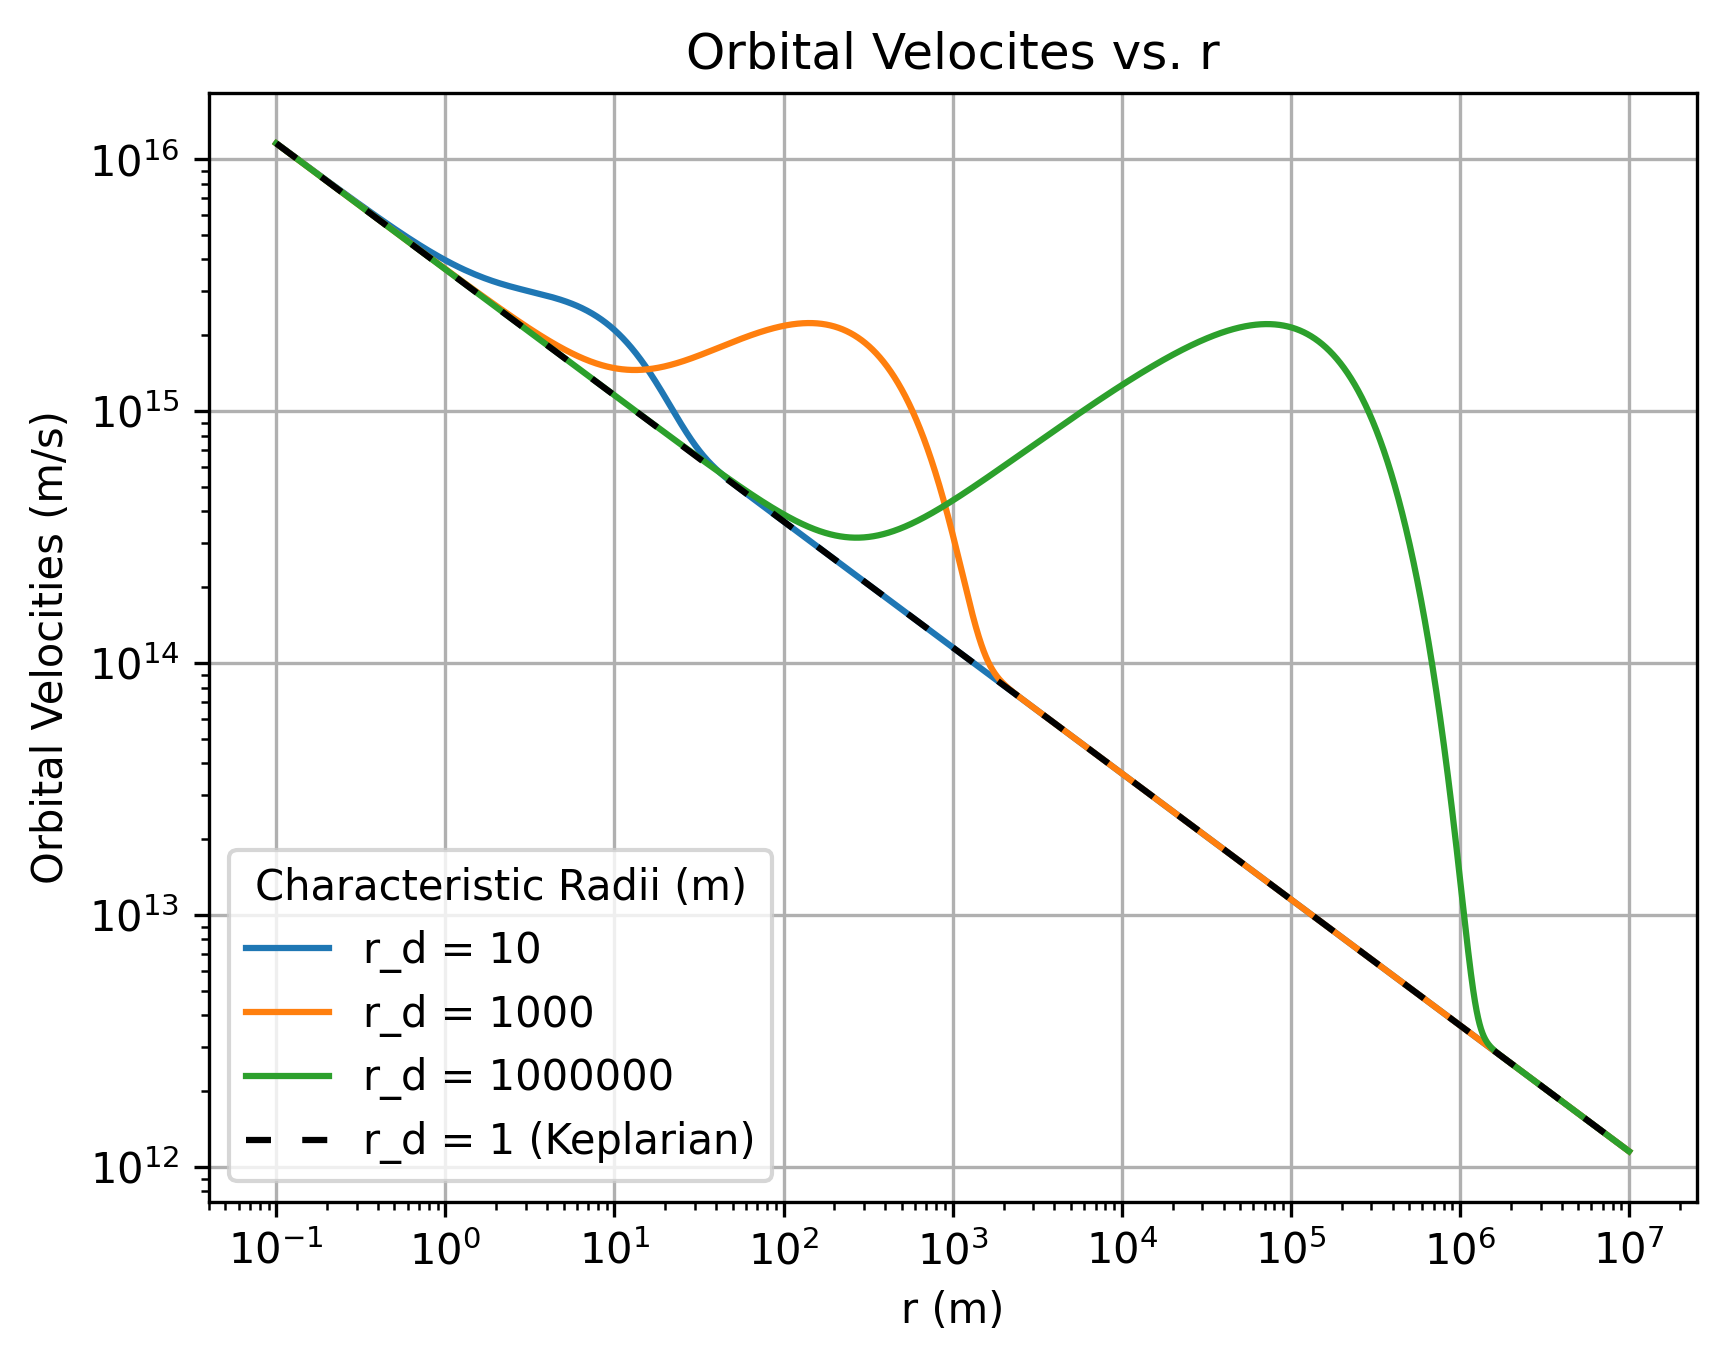
\includegraphics[scale=0.75]{figures/graph_orbvelVr.png}
    \caption{Plot of Orbital Velocities vs. $r$}
    \label{fig:graph_orbvelVr}
\end{figure}
the modified orbital velocity tends to the Keplerian expectation for large or small $r$, but around $r_d$ the orbital velocity has a bump (FIG.~\ref{fig:graph_orbvelVr}). Observations of orbital velocities show that velocities do not fall off purely exponentially as is the Keplerian expectation, but rather flatten out at some distance near the outer edges of the galactic spiral~\cite{navarro_1997,brownstein_2006}. The bump in orbital velocity calculated with corrections ought align with the cosmological observations for the right choice of $r_d$. D'Agostino et al. demonstrate that the observed galactic rotation curves of the Milky Way and M31 (Andromeda) can be consistently explained within a Yukawa-modified gravitational framework, without invoking dark matter. Moreover, D'Agostino et al. highlight that the Yukawa scale length is constrained to be of order $\sim$kpc ($r_d=0.740^{+0.082-0.088}$kpc), setting a fundamental limit on its precise determination from galactic-scale data \cite{dagostino_2024}.

\section{This Model of Gravity as a Gauge Theory}
I would like to take this opportunity to present a brief review of the model presented and its comparison to the differential geometry of Standard Model gauge theory, highlighting why it might be better prepared for quantization compared to cannonical GR. This model reframes gravity in terms of the affine connection as the fundamental field, with the curvature tensor serving as the field strength. This approach bears striking similarities to the gauge theories of the Standard Model. In this model, the gravitational potential is represented by the affine connection $\Gamma$, analogous to the gauge potential $A$ in Yang-Mills theories~\cite{peskin_1995,hauser_2019_1,hauser_2019_2,hauser_2019_3}. The curvature tensor $R$ serves as the gravitational field strength, similar to the field strength tensor $F$ in gauge theories. The equations based on the squared norm of the field strength ($\mathcal{R}^\alpha_{\mu\beta\nu}\mathcal{R}_\alpha^{\mu\beta\nu}$), mirrors the Yang-Mills action ($F^{a}_{\mu\nu} F_{a}^{\mu\nu}$)~\cite{peskin_1995}.

This formulation offers several advantages for quantization. The model naturally incorporates the geometric nature of gravity while maintaining a structure similar to other quantum field theories. The squared field strength in the action is a promising starting point for renormalization, as it is of the same form as renormalizable gauge theories. The model respects general coordinate invariance, analogous to gauge invariance in the Standard Model~\cite{hauser_2019_1,hauser_2019_2,hauser_2019_3}. The background field method used in this model ($g_{ab} = \eta_{ab} + h_{ab}$) is well-suited for perturbative quantum calculations~\cite{bern_2002}. This approach potentially allows for a more unified treatment of gravity with other fundamental forces.

In contrast, GR's action (based on the Ricci scalar $R$) and its direct quantization face several challenges. GR is notoriously difficult to renormalize due to its non-polynomial dependence on the metric~\cite{deser_2009}. Traditional approaches to quantizing GR often struggle with background independence~\cite{reuter_2009,ashtekar_2009,ashtekar_2004,read_2023}. Perturbative expansions in GR can lead to divergences that are challenging to handle~\cite{deser_1957}. This model's closer alignment with the structure of gauge theories potentially offers a more promising path towards a quantum theory of gravity, addressing some of the key obstacles faced in quantizing GR directly.

\section*{Conclusions}
In this work I have shown that by reframing the gravitational field in the spirit of Poplawski by treating the affine connection as the fundamental dynamical variable and taking the curvature tensor as the field strength, using an action built from the squared norm of that field strength, $S=\int{R_{abcd}R^{abcd}D^4x}$, deriving the Euler–Lagrange equations for the connection and, by varying the metric, obtaining the metric field equations (Eq. 16), working with a background-field decomposition $g_{ab}=\eta_{ab}+h_{ab}$, and carrying out a linearized analysis about a maximally symmetric background, the canonical Einstein field equations re-emerge as a limiting (weak-field / small-local-curvature) approximation of the full theory. In other words, standard GR appears as the low-order approximation of a broader geometric framework rather than as the unique description of gravity at all scales.

The fuller gravitational equations contain corrections to the Einsteinian description. On cosmological (global) scales the extra geometric terms behave like an effective cosmological constant giving a small, positive effective curvature consistent with the observed accelerated expansion. Thus the model provides a purely geometric mechanism that can reproduce the phenomenology normally attributed to dark energy without introducing an ad hoc vacuum term. On local (galactic) scales the linearized equations around a spherically symmetric background produce a Yukawa-type modification of the Schwarzschild solution and a modified Newtonian potential of the form $\Phi(r) = -\frac{GM}{r} - G M e^{-\frac{\ln(r_d)}{r_d} r}$. The characteristic length scale $r_d$ can be made consistent with the findings of D'Agostino which showed the Yukawa correction can account for the flattening of galactic rotation curves without dark-matter halos when $r_d=0.740^{+0.082-0.088}$kpc.

In summary, the affine, squared-curvature formulation reproduces Einstein’s field equations in the appropriate limit, produces geometric corrections that can account for accelerated expansion and galaxy rotation-curve anomalies without introducing new forms of matter or energy, and offers a promising route toward a modern field-theoretic description of gravity. These results mean dark matter and dark energy are not be required in a modern model of gravity.

\appendix

\begin{fleqn}
\section{Derivation of the Metric Field Equations of the Squared Norm}\label{app.derv_metric_field_eqs}
\begin{equation*}
\begin{aligned}
    \mathcal{L} &= \mathcal{R}_{abcd} \mathcal{R}^{abcd} \\
    \delta \mathcal{L} &= 2 \delta \mathcal{R}_{abcd} \cdot \mathcal{R}^{abcd}
\end{aligned}
\end{equation*}
\begin{equation*}
\begin{aligned}
    \delta \mathcal{R}_{abcd} &= D_c \delta \Gamma_{abd} - D_d \delta \Gamma_{abc} \\
    \delta \Gamma_{abc} &= \frac{1}{2} \delta(\partial_a g_{bc} + \partial_b g_{ca} - 2 \partial_c g_{ab}) \\
    \delta (\partial_a g_{bc}) &= D_a \delta g_{bc} \\
\end{aligned}
\end{equation*}
substitute this into $\delta \mathcal{L}$,
\begin{align*}
    \delta \mathcal{L} &= 2\left( \frac{1}{2} D_c (D_a \delta g_{bd} - D_b \delta g_{da} - 2 D_d \delta g_{ab}) - \frac{1}{2} D_d (D_a \delta g_{bc} - D_b \delta g_{da} - 2 D_c \delta g_{ab}) \right) \mathcal{R}^{abcd} \\
    &= \left( D_c (D_a \delta g_{bd} - D_b \delta g_{da} - 2 D_d \delta g_{ab}) - D_d (D_a \delta g_{bc} - D_b \delta g_{da} - 2 D_c \delta g_{ab}) \right) \mathcal{R}^{abcd}
\end{align*}
to get similar indices and pull out a variation of the metric tensor let us make the substitution (note that $\mathds{1}$ is an identity matrix): $D_c D_a \delta g_{bd} \rightarrow (\mathds{1}^n_b \mathds{1}^m_d D_c D_a) \delta g_{nm}$,
\begin{equation*}
    \delta \mathcal{L} = \left( D_c (\mathds{1}^n_b \mathds{1}^m_d D_a + \mathds{1}^n_d \mathds{1}^m_a D_b - 2 \cdot \mathds{1}^n_a \mathds{1}^m_b D_d) - D_d (\mathds{1}^n_b \mathds{1}^m_c D_a + \mathds{1}^n_c \mathds{1}^m_a D_b - 2 \cdot \mathds{1}^n_a \mathds{1}^m_b D_c) \right) \delta g_{nm} \mathcal{R}^{abcd}
\end{equation*}
remembering this is all taking place under an integral we can use integration by parts to change from a derivative of $\delta g_{nm}$ to a derivative of $\mathcal{R}^{abcd}$,
\begin{equation*}
    \delta \mathcal{L} = \left( \left( D_c (\mathds{1}^n_b \mathds{1}^m_d D_a + \mathds{1}^n_d \mathds{1}^m_a D_b - 2 \cdot \mathds{1}^n_a \mathds{1}^m_b D_d) - D_d (\mathds{1}^n_b \mathds{1}^m_c D_a + \mathds{1}^n_c \mathds{1}^m_a D_b - 2 \cdot \mathds{1}^n_a \mathds{1}^m_b D_c) \right) \mathcal{R}^{abcd} \right) \delta g_{nm}
\end{equation*}
\begin{equation*}
    \frac{\delta \mathcal{L}}{\delta g_{nm}} = \left( \left( D_c (\mathds{1}^n_b \mathds{1}^m_d D_a + \mathds{1}^n_d \mathds{1}^m_a D_b - 2 \cdot \mathds{1}^n_a \mathds{1}^m_b D_d) - D_d (\mathds{1}^n_b \mathds{1}^m_c D_a + \mathds{1}^n_c \mathds{1}^m_a D_b - 2 \cdot \mathds{1}^n_a \mathds{1}^m_b D_c) \right) \mathcal{R}^{abcd} \right)
\end{equation*}
distributing $\mathcal{R}^{abcd}$,
\begin{equation*}
\begin{aligned}
    \frac{\delta \mathcal{L}}{\delta g_{nm}} = &D_c \mathds{1}^n_b \mathds{1}^m_d D_a \mathcal{R}^{abcd} + D_c \mathds{1}^n_d \mathds{1}^m_a D_b \mathcal{R}^{abcd} - 2 D_c \mathds{1}^n_a \mathds{1}^m_b D_d \mathcal{R}^{abcd} \\
    &- D_d \mathds{1}^n_b \mathds{1}^m_c D_a \mathcal{R}^{abcd} - D_d \mathds{1}^n_c \mathds{1}^m_a D_b \mathcal{R}^{abcd} + 2 D_d \mathds{1}^n_a \mathds{1}^m_b D_c \mathcal{R}^{abcd} \\
    = &D_c D_a \mathcal{R}^{ancm} + D_c D_b \mathcal{R}^{mbcn} - 2 D_c D_d \mathcal{R}^{nmcd} \\
    &- D_d D_a \mathcal{R}^{anmd} - D_d D_b \mathcal{R}^{mbnd} + 2 D_d D_c \mathcal{R}^{nmcd}
\end{aligned}
\end{equation*}
reordering some indices and observing symmetries of the Riemann tensor,
\begin{equation*}
\begin{aligned}
    \frac{\delta \mathcal{L}}{\delta g_{nm}} = &D_b D_a \mathcal{R}^{namb} - D_b D_a \mathcal{R}^{manb} - 2 D_a D_b \mathcal{R}^{nmab} \\
    &+ D_b D_a \mathcal{R}^{namb} - D_a D_b \mathcal{R}^{mbna} + 2 D_b D_a \mathcal{R}^{nmab}
\end{aligned}
\end{equation*}
\begin{equation*}
\begin{aligned}
    \frac{\delta \mathcal{L}}{\delta g_{nm}} &=
    \left( D_b D_a \mathcal{R}^{namb} + D_b D_a \mathcal{R}^{namb} \right)
    - \left( D_b D_a \mathcal{R}^{manb}  - D_a D_b \mathcal{R}^{mbna}\right)
    - \left( 2 D_a D_b \mathcal{R}^{nmab} + 2 D_b D_a \mathcal{R}^{nmab} \right) \\
    &= 2 D_b D_a \mathcal{R}^{namb} - 2 D_b D_a \mathcal{R}^{manb} - 2 D_{[a} D_{b]} \mathcal{R}^{nmab} \\
    &= -2 D_{[b} D_{a]} \mathcal{R}^{namb} - 2 D_{[a} D_{b]} \mathcal{R}^{nmab} \\
    &= - 2 D_{[a} D_{b]} \left( \mathcal{R}^{namb} + \mathcal{R}^{nmab} \right)
\end{aligned}
\end{equation*}
\begin{equation*}
    D_{[a} D_{b]} \mathcal{R}^{namb} = -\frac{1}{2} \mathcal{R}_{ab}\mathcal{R}^{namb}
\end{equation*}
\begin{equation*}
\boxed{
    \frac{\delta \mathcal{L}}{\delta g_{nm}} = \mathcal{R}_{ab} \mathcal{R}^{namb} + 2 D_{[a} D_{b]} \mathcal{R}^{nmab}
}
\end{equation*}
\end{fleqn}

\bibliographystyle{apsrev4-2} % APS PRD style
\bibliography{On_The_Dynamics_Of_The_Gravitational_Field_And_Higher_Order_Field_Equations}

\end{document}